\documentclass{article}

\usepackage{tikz}
\usepackage{tikz}
\usepackage{pgfplots}
\usetikzlibrary{backgrounds, positioning, fit}
\usetikzlibrary{shapes.geometric}
\usetikzlibrary{patterns}

%% put tikzlibrary below if necessary

% set up externalization
\usetikzlibrary{external}
\tikzset{external/system call={latex \tikzexternalcheckshellescape -halt-on-error
-interaction=batchmode -jobname "\image" "\texsource";
dvips -o "\image".ps "\image".dvi;
ps2eps "\image.ps"}}
\tikzexternalize



\begin{document}

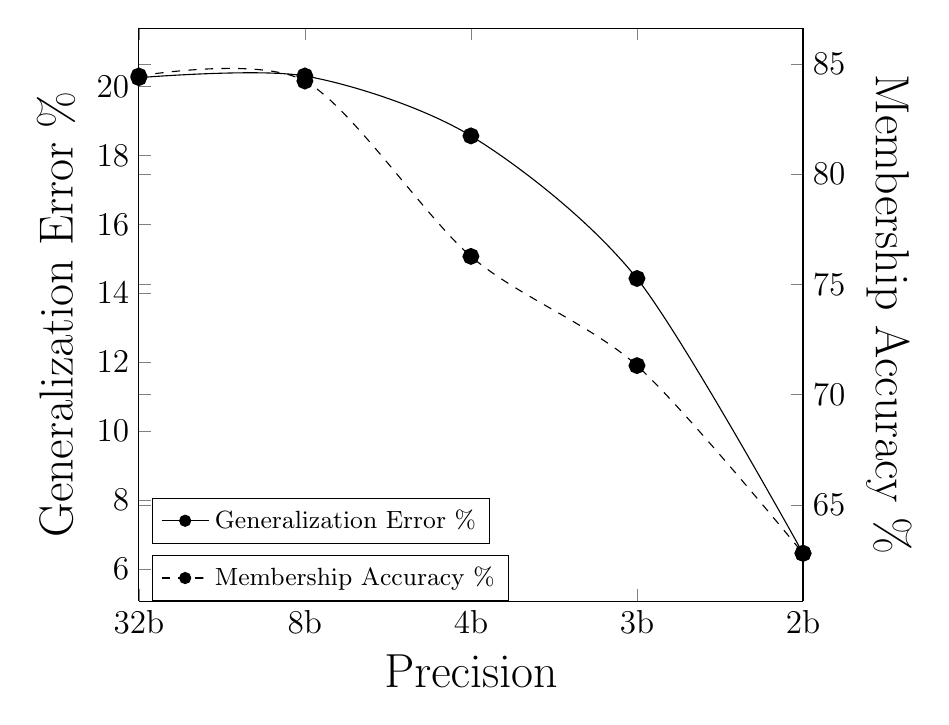
\begin{tikzpicture}
% let both axes use the same layers
\pgfplotsset{set layers}
%
\begin{axis}[
%title={(b) Purchase},
%title style={at={(0.5,0)},anchor=north,yshift=-40, font=\huge},
scale only axis,
line width=2.0pt,
mark size=2.0pt,
xmin=0,xmax=4,
ylabel={Generalization Error \%},
axis y line*=left,
xlabel={Precision},
xtick={0,1,2,3,4},
xlabel style={font=\LARGE},
ylabel style = {font=\LARGE},
xticklabel style = {font=\large},
yticklabel style = {font=\large},
xticklabels={32b, 8b, 4b, 3b, 2b},
legend style={at={(0.02,0.1)},anchor=south west, font=\small}
]
\addplot[
    color=black,
    solid,
    mark=*,
    mark options={solid},
    smooth
    ]
    coordinates {
    (0,20.26)(1,20.31)(2,18.57)(3,14.43)(4,6.45)
      };
      \addlegendimage{color=black,solid,mark=*, mark options={solid}}
      \addlegendentry{Generalization Error \%}
\end{axis}

\begin{axis}[
scale only axis,
line width=2.0pt,
mark size=2.0pt,
xmin=0,xmax=4,
ylabel near ticks, yticklabel pos=right,
ylabel={Membership Accuracy \%},
ylabel style = {rotate=180,font=\LARGE},
yticklabel style = {font=\large},
axis x line=none,
legend style={at={(0.02,0)},anchor=south west, font=\small}
]
\addplot[
    color=black,
    dashed,
    mark=*,
    mark options={solid},
    smooth
    ]
    coordinates {
    %(0,62.08)(1,62.05)(2,59.86)(3,57.27)(4,53.38)
    (0,84.45)(1,84.22)(2,76.27)(3,71.32)(4,62.81) %updated results
        };
        \addlegendimage{color=black,dashed,mark=*,mark options={solid}}
        \addlegendentry{Membership Accuracy \%}
\end{axis}
\end{tikzpicture}


\end{document}
